To accelerate the computation, several approaches were tried. For example, Ahmed \emph{et al.} used a dedicated FPGA (\emph{Field Programmable Gate Array}) to accelerate the research with the FM-index and the extension~\cite{Ahmed:FPGA}. Another approach from Mashtaq \emph{et al.} consisted in streaming DNA sequences alignment tasks to a cluster with Apache Spark~\cite{Mushtaq:spark}. But these solutions require extra hardware and can be difficult to set up. We would like to propose a solution using common hardware found on computers, in particular, Graphics Processing Units, or GPUs.

DNA computation can take advantage of the inner structure of a GPU to compute the alignment faster. First, we will quickly recap the current solutions at hand. Then a presentation of the GPU architecture and programming paradigm will show how this device work and how they are adapted for this work.

\subsection{Parallel computing for DNA alignment}

The computation for alignment between two DNA strings is intensive, yet simple. The main problem comes from the input data size. Still, it is important to note that each pair of alignment is independent from the others. A simple and effective way to accelerate the computation is to parallelise it. On a computer, one can use multiple threads on a CPU to achieve that parallelisation and compute several alignments at the same time. However, the number of threads available on a CPU is limited to a dozen, or a few dozen at best; but Graphics Computing Units (GPUs) can have hundreds to thousands of cores at disposal. This makes GPUs a hardware of choice for acceleration using parallel computing. Running multiple alignments in parallel is called \emph{inter-sequence parallelisation}. 

It is possible to go even further with \emph{intra-sequence parallelisation}, that is, to calculate the dynamic programming matrix with multiple threads. This implies having synchronisation phases: since the cell values depends on the previously calculated ones, it implies processing with a logic order, and require a high level of optimisation for efficient speed-up~\cite{Houtgast:gpu-accelerated}. However, we will not explore this topic later on.

As for current solutions, a quick list of some of the existing software for DNA alignment will be presented. These tools are most often present as libraries, to be able to integrate them in bigger and more easy-to-use software.

\begin{itemize}
    \item \emph{SeqAn}~\cite{Doring:seqan} is a C++ toolbox for DNA alignment. It features a lot of various tools, and implements its own C++ library for alignment. It runs on multiple CPU threads, and can rely on SIMD for moderate acceleration,
    \item \emph{Basic Local Alignment Seach Tool} (\emph{BLAST})~\cite{Altschul:BLAST} searches for pairwise alignment with the seed-extension method,
    \item \emph{Burrows-Wheeler Aligner} (\emph{BWA})~\cite{li:bwa} is a DNA aligner focused on speed relying on FM-index for seeding, with BLAST-like extension,
    \item \emph{NVBIO}~\cite{nvidia:nvbio} is a GPU-accelerated library written in CUDA, the dedicated language for general-purpose GPU computing on NVIDIA GPUs. It has a lot of features including banded dynamic programming, fast FM-index construction, and efficient data handling between CPU and GPU,
    \item \emph{GASAL2}~\cite{Ahmed:gasal2} is also a CUDA-written library for DNA alignment, developed with speed in mind. Despite its relatively small number of features, it runs all compute-intensive parts on GPU for maximum speed-up.
\end{itemize}

Today, there are a lot of alignment software available~\cite{wiki:ListAlignmentSoft} and for the rest of the thesis, we will focus on BWA.

\subsection{General-purpose GPU computing basics}

Historically, GPUs have been developed to render graphics, and because of this purpose, have a highly parallel architecture to cope with independent parts of the picture. GPUs now can be used for generic computing, as a separate accelerator towards which the CPU can offload parts of the calculation. As such, they can spawn a high number of threads, with an order of magnitude bigger than CPUs (several thousands versus a few dozen), although their clock speed is slower (Around 1 to 2 GHz while regular CPUs can reach 4 to 5GHz). We introduce the terms \emph{host} to designate the CPU-side of the machine, constituted of the CPU and its RAM; and \emph{device} the GPU-side with its dedicated onboard memory called \emph{global memory} or \emph{VRAM}, short for Video RAM. Figure~\ref{fig:gpu-arch} shows a summarized view of the CPU-GPU tandem. The CPU "host" triggers launches of parallel functions called \emph{kernels} on the GPU. This kernel is launched on a \emph{grid}, divided into \emph{blocks}, each of them having a certain number of \emph{threads}. The grid and block sizes are specified as launch parameters, and they are adapted to divide all the data to process into a suited number of threads. Inside a block, threads can access a shared memory. Scopes from different memories are specified on Figure~\ref{fig:gpu-memory-scope}.

\begin{figure}[h]
	\centering
	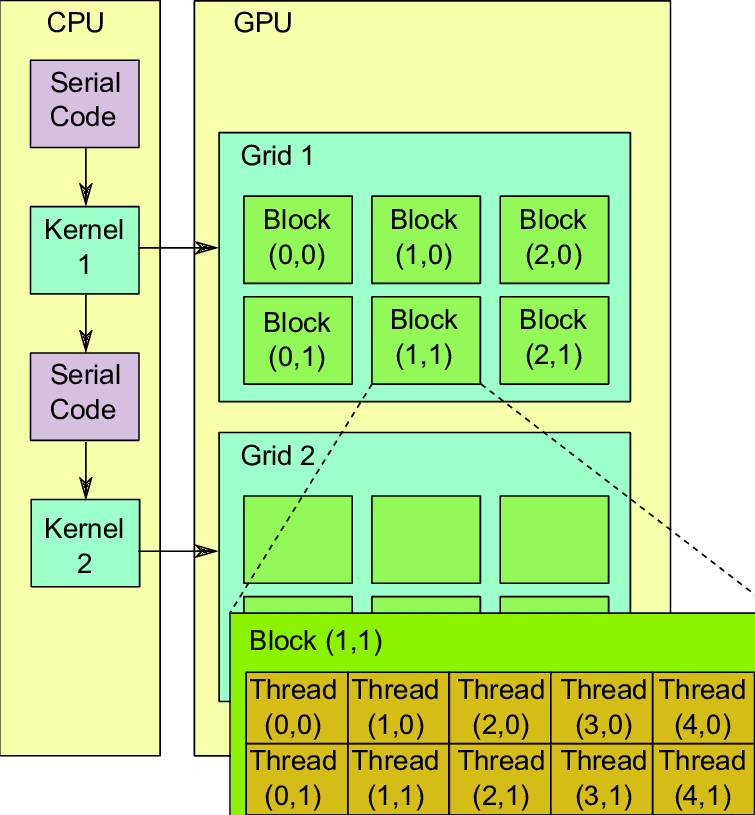
\includegraphics[width=0.6\linewidth]{gpu-arch}
	\caption{GPU architecture schematics (from~\cite{Bartezzaghi:gpu-arch})}
	\label{fig:gpu-arch}
\end{figure}


\begin{figure}[h]
	\centering
	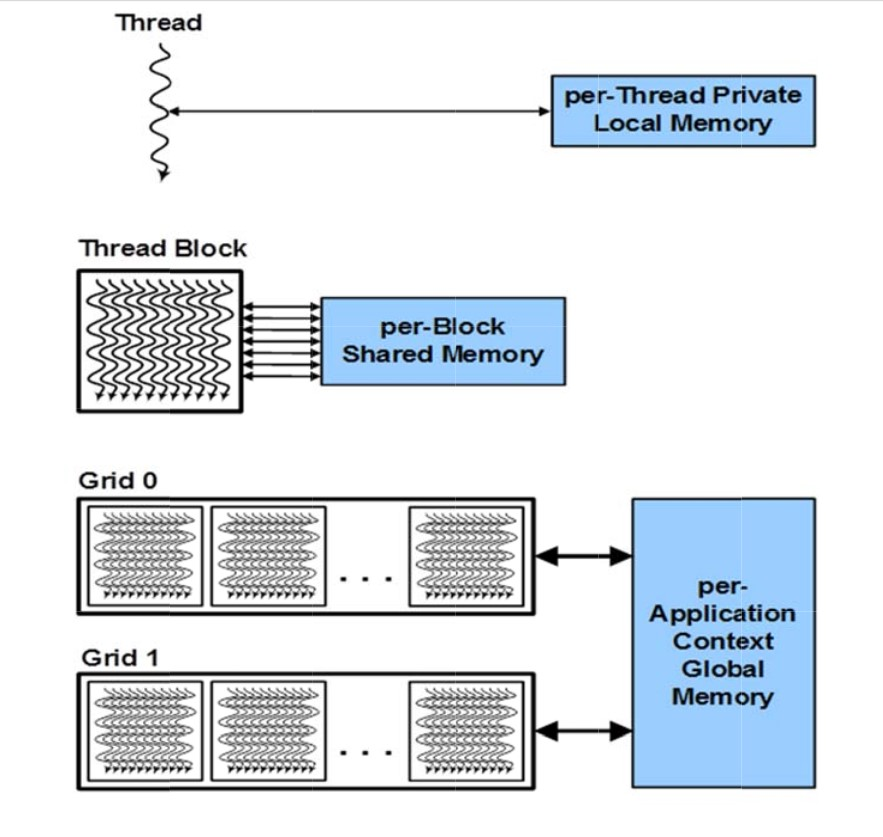
\includegraphics[width=0.6\linewidth]{gpu-memory-scope}
	\caption{GPU memories scope (from~\cite{nvidia:keplerarch})}
	\label{fig:gpu-memory-scope}
\end{figure}


This presents two main benefits. First, some problems that can be highly parallelizable will take advantage of the huge thread number of a GPU. Second, being able to offload the calculation to a separate device means that both the CPU and the GPU can be busy at the same time: this enables hidden-time computation, that is, the CPU can continue to work on another part of the code while the GPU runs its part, and the former can retrieve the results only when the latter is done.

This hidden time capability is achieved thanks to non-blocking launches and streams. For several years now, it is possible to launch multiple threads of the same function on the GPU, called \emph{kernel}, without needing to wait for all threads to finish. The kernel call directly returns, and the host can simply check when needed (periodically) if the GPU is done. When a program declares two streams, the host can launch the kernel on Stream~\#1, then fill up the data for Stream~\#2 while the first one computes. When Stream~\#2 is launched, by that time, Stream~\#1 has finished, so results can be retrieved and Stream~\#1 can be filled again with the next data to compute while Stream~\#2 computes; and so on.

It is crucial to monitor some metrics to ensure the GPU is used to its fullest, and has its own limited resources. We can mention:

\begin{itemize}
	\item occupation (in \%): it represents how much of the computing resources are used,
	\item VRAM use (in MB): it is the onboard memory and cannot exceed the hardware resources,
	\item data transfer time: since it is a separate device, it is important to check if data transfers are taking more or less time than the computation part.
\end{itemize}
